%\title{emnlp 2017 instructions}
% File emnlp2017.tex
%

\documentclass[11pt,letterpaper]{article}
\usepackage{emnlp2017}
\usepackage{times}
\usepackage{latexsym}
\usepackage{todonotes}
\usepackage{url}
\usepackage{blindtext}
\usepackage{fancybox, graphicx}
\usepackage{booktabs}
\usepackage{multirow}
\usepackage{arydshln}
\usepackage{pgf-pie}
\usepackage{float}

% Uncomment this line for the final submission:
%\emnlpfinalcopy

%  Enter the EMNLP Paper ID here:
\def\emnlppaperid{388}

% To expand the titlebox for more authors, uncomment
% below and set accordingly.
% \addtolength\titlebox{.5in}    

\newcommand\BibTeX{B{\sc ib}\TeX}

%%% Consistency
\newcommand{\ex}[1]{``\emph{#1}''}
\newcommand{\ann}[2]{#1$_{#2}$}
\newcommand{\brand}[1]{{\tt #1}}
\newcommand{\dbpedia}[0]{DBpedia}
\newcommand{\triplet}[3]{(#1, \textbf{#2}, {#3})}
\newcommand{\aap}[0]{\brand{Ask a Patient}}
\newcommand{\keras}[0]{Keras}
\newcommand{\tensorflow}[0]{TensorFlow}
\newcommand{\wv}[0]{Word2Vec}
\newcommand{\rascal}[0]{RASCAL}
\newcommand{\oie}[0]{Open IE}
\newcommand{\sent}[1]{``\emph{#1}''}
\newcommand{\pred}[1]{\textbf{#1}}
\newcommand{\extraction}[3]{(#1; \pred{#2}; #3)}
\newcommand{\oielabel}[1]{\fontsize{12}{10}\selectfont #1}
%\newcommand{\oielabel}[1]{\scriptsize {\textbf{\emph{#1}}}}-

% Placeholders

\newcommand{\blindfig}[2]{
  \begin{figure}[ht]
    \resizebox{1\columnwidth}{!}{
      
\includegraphics{figure-file}
    }
    \caption{#1 (placeholder)}
    \label{#2}
  \end{figure}
}

\newcommand{\Blindfig}[2]{
  \begin{figure*}[ht]
    \resizebox{1\textwidth}{!}{
      
\includegraphics{figure-file}
    }
    \caption{#1 (placeholder)}
    \label{#2}
  \end{figure*}
}


% Misc
\newcommand*\samethanks[1][\value{footnote}]{\footnotemark[#1]}

\title{Supervised Open Information Extraction}

% Author information can be set in various styles:
% For several authors from the same institution:
% \author{Author 1 \and ... \and Author n \\
%         Address line \\ ... \\ Address line}
% if the names do not fit well on one line use
%         Author 1 \\ {\bf Author 2} \\ ... \\ {\bf Author n} \\
% For authors from different institutions:
% \author{Author 1 \\ Address line \\  ... \\ Address line
%         \And  ... \And
%         Author n \\ Address line \\ ... \\ Address line}
% To start a seperate ``row'' of authors use \AND, as in
% \author{Author 1 \\ Address line \\  ... \\ Address line
%         \AND
%         Author 2 \\ Address line \\ ... \\ Address line \And
%         Author 3 \\ Address line \\ ... \\ Address line}
% If the title and author information does not fit in the area allocated,
% place \setlength\titlebox{<new height>} right after
% at the top, where <new height> can be something larger than 2.25in
\author{Siddharth Patwardhan \and Preethi Raghavan \\
  {\tt publication@emnlp2017.net}}

\date{}

\begin{document}

\maketitle

\begin{abstract}
  Open Information Extraction (Open IE) has gained popularity as an underlying representation in a
  wide array of semantic applications.
  However, the lack of a large gold standard corpus for Open IE has
  limited the development of automatic extraction techniques to largely rule-based algorithms.
  In a recent advancement, a first large Open IE corpus for verbal predicates was presented, which ``opens the door'' for applying modern machine learning techniques for this task.
  In this paper, we utilize this corpus to develop a first supervised Open IE extractor.
  As this is the first supervised Open IE system,
  we use a deep bi-LSTM transducer, proven to be useful in similar tasks, and focus on laying the basic building blocks needed for supervised Open IE: encoding, decoding, confidence estimation, and proper error analysis.
  Our evaluation shows that the new extractor significantly outperforms
  the currently most prominent Open IE systems.
\end{abstract}

\section{Introduction}
\label{sec:introduction}
Open Information Extraction (Open IE)
was presented as an open variant of the traditional ``closed'' information extraction task \cite{etzioni2008open}.
It aims to extract coherent standalone propositions, asserted by the sentence.
For example, given the sentence
\sent{The president congratulated the Cubs, a Chicago based baseball team, who won the World Series},
the following are valid Open IE propositions:
\begin{enumerate}
\item \extraction{The president}{congratulated}{the Cubs}
\item \extraction{The president}{congratulated}{a Chicago based baseball team}
\item \extraction{The cubs}{won}{the World Series}
\item \extraction{a Chicago based baseball team}{won}{the World Series}
\end{enumerate}
Each Open IE proposition is a tuple consisting of a single predicate slot (in bold), and an arbitrary number of arguments (separated by a semicolon).

Since its inception, Open IE has garnered popularity among researchers, who leveraged  its simple yet robust representation for various semantic tasks.
For example, Open IE has been used as an underlying representation in knowledge base population \cite{2015angeli-openie}, question answering \cite{fader2014open}
textual entailment \cite{Berant:ACL11} and more \cite{Melamud:ACL13,yang2016peak}.

In spite of this wide attention, up until recently there was no large gold reference corpus for Open IE,
which inhibited the use of modern machine learning techniques for the task.
The developed extractors therefore used either a semi-supervised approach \cite{wu2010open,banko2007open}, or, more prominently, rule-based algorithms to extract predicate-argument structures over part-of-speech tags \cite{fader2011identifying} or  dependency trees \cite{mausam2012open,del2013clausie,props2016}.
More recently, Open IE4\footnote{\url{https://github.com/allenai/openie-standalone}} adopted this paradigm and extracted Open IE propositions from predicted Semantic Role Labeling (SRL)
annotations.

%% Open IE4's ability to efficiently extract Open IE from SRL annotations is largely
%% thanks to the similarities between the tasks.
%% In particular, both SRL and Open IE try to extract predicate-argument tuples stated verbatim the text,
%% however SRL also grounds each predicate using a predefined lexicon \cite{propbank}, and does not attempt
%% to extract asserted or minimal propositions. 

Recently, \citet{Stanovsky2016EMNLP} %used this observation and 
presented a first large gold standard corpus of Open IE extractions for verbal predicates, automatically converted from a large QA-SRL corpus (a variant of SRL, \cite{hequestion}).
In addition, they tested the performance of several Open IE extractors and found that
in spite of their robustness,
all of them lack in precision and recall.

Following the creation of this Open IE corpus,
we present here a first supervised model for Open IE.
%Using a large training corpus we can harness the latest advancements in supervised machine learning for the task of
%Open IE.
%In particular, we focus this work on the challenges in fitting this task for an RNN framework.
We focus this work on formalizing Open IE for deep neural networks and re-frame it as a \emph{word transduction} task, providing novel solutions for label encoding, decoding,
and confidence estimation.
Since we focus on devising the overall framework, we use a rather simple bi-LSTM transducer model,
inspired by the recent state-of-the-art models for supervised SRL.
Nevertheless, we find that this model surpasses all previous Open IE systems and
offers a better precision-recall trade-off.

%% We hope that this first supervised model, made publicly available upon publication,  will be useful for semantic applications as a state of the art Open IE extractor, and will serve as the basis for further exploration of machine learning techniques for this task.




\section{Background: Open Information Extraction}
\label{sec:background}
%% \begin{itemize}
%% \item Describe the task (list briefly its principles)
%% \item Give examples.
%% \end{itemize}
% Please add the following required packages to your document preamble:
%



\begin{table*}[tb!]
  \centering
  \resizebox{1\textwidth}{!}{
    \begin{tabular}{@{}l@{}}
      \toprule
      \textbf{OIE Encoding Examples}  \\ \midrule
         \sent{The president claimed that he won the majority vote} \\
         \begin{tabular}[c]{@{}l@{}}
           \extraction{The president}{claimed that he won}{the majority vote}  \\\cdashline{1-1}
\small{           \ann{The}{A0-B} \ann{president}{A0-I} \ann{claimed}{P-B} \ann{that}{P-I} \ann{he}{P-I} \ann{won}{P-I}
           \ann{the}{A1-B} \ann{majority}{A1-I} \ann{vote}{A1-I}}
         \end{tabular} \\\hline

         \sent{Barack Obama, a former U.S president, was born in Hawaii} \\
         \begin{tabular}[c]{@{}l@{}}
           \extraction{Barack Obama}{was born in}{Hawaii}  \\
           \extraction{a former U.S. president}{was born in}{Hawaii} \\\cdashline{1-1}
\small{           \ann{Barack}{A0-B} \ann{Obama}{A0-I} \ann{,}{O} \ann{a}{O} \ann{former}{O} \ann{U.S.}{O} \ann{president}{O} \ann{,}{O} \ann{was}{P-B} \ann{born}{P-I} \ann{in}{P-I} \ann{Hawaii}{A1-B} }\\
\small{           \ann{Barack}{O} \ann{Obama}{O} \ann{,}{O} \ann{a}{A0-B} \ann{former}{A0-I} \ann{U.S.}{A0-I} \ann{president}{A0-I} \ann{,}{O} \ann{was}{P-B} \ann{born}{P-I} \ann{in}{P-I} \ann{Hawaii}{A1-B}}
         \end{tabular} \\\hline

%%          \sent{Russian plane was carrying ammunition for Syria} \\
%%          \begin{tabular}[c]{@{}l@{}}
%%           (Russian plane; \pred{was carrying}; ammunition; for Syria) \\\cdashline{1-1}
%% \small{           \ann{Russian}{A0-B} \ann{plane}{A0-I} \ann{was}{P-B} \ann{carrying}{P-I} \ann{ammunition}{A1-B}
%%            \ann{for}{A2-B} \ann{Syria}{A2-I}}
%%          \end{tabular} \\\hline

%%          \sent{Obama sends note to Russia about the hacking} \\
%%          \begin{tabular}[c]{@{}l@{}}
%%            (Obama; \pred{sends note}; to Russia; about the hacking) \\\cdashline{1-1}
%% \small{           \ann{Obama}{A0-B} \ann{sends}{P-B} \ann{note}{P-I} \ann{to}{A1-B} \ann{Russia}{A1-I} \ann{about}{A2-B} \ann{the}{A2-I} \ann{hacking}{A2-I}}
%%          \end{tabular} \\\hline

         \sent{Theresa May plans for Brexit, on which the UK has voted on last June} \\
         \begin{tabular}[c]{@{}l@{}}
           (Theresa May; \pred{plans for}; Brexit) \\
           (the UK; \pred{has voted on}; Brexit; last June) \\\cdashline{1-1}
           \small{           \ann{Theresa}{A0-B} \ann{May}{A0-I} \ann{plans}{P-B} \ann{for}{P-I} \ann{Brexit}{A1-B} \ann{,}{O} \ann{on}{O} \ann{which}{O} \ann{the}{O} \ann{UK}{O} \ann{has}{O} \ann{voted}{O} \ann{on}{O} \ann{last}{O} \ann{June}{O}}\\
     \small{\ann{Theresa}{O} \ann{May}{O} \ann{plans}{O} \ann{for}{O} \ann{Brexit}{A1-B} \ann{,}{O} \ann{on}{O} \ann{which}{O} \ann{the}{A0-B} \ann{UK}{A0-I} \ann{has}{P-B} \ann{voted}{P-I} \ann{on}{P-I} \ann{last}{A2-B} \ann{June}{A2-I}}

         \end{tabular} \\

       \bottomrule
      \end{tabular}
  }
  \caption{Example sentences and respective Open IE extractions.
    The corresponding encodings are presented below the dashed lines, where subscripts indicate the associated
    BIO label.}
  \label{tab:oie_examples}
  \end{table*}



%% \begin{figure*}[tb!]
%% %  \vspace{-1\baselineskip}
%%   \framebox{\parbox{\dimexpr\linewidth-2\fboxsep-2\fboxrule}{
%%       \begin{enumerate}
%%         \item
%%          \sent{The president claimed that he won the majority vote}\\
%%          \extraction{The president}{claimed that he won}{the majority vote}
%%        \item
%%          \sent{Barack Obama, a former U.S president, was born in Hawaii}\\
%%          \extraction{Barack Obama}{was born in}{Hawaii}\\
%%          \extraction{a former U.S. president}{was born in}{Hawaii}
%%        \item
%%          \sent{Russian plane was carrying ammunition for the Syrian government}\\
%%          (Russian plane; \pred{was carrying}; ammunition; for the Syrian government)
%%        \item
%%          \sent{Obama administration sends note to Russia regarding alleged hacking}\\
%%          (Obama administration; \pred{sends note}; to Russia; regarding alleged hacking)
%%       \end{enumerate}
%%   }}
%%   \caption{Example sentences and respective Open IE extractions.}
%%   \label{fig:oie_examples}
%% \end{figure*}
%% \todo{Figure \ref{fig:oie_examples}: Should we add the corresponding SRL structures?}

The task of Open IE focuses on extracting stand-alone propositions (predicate and arguments tuples)
which are explicitly asserted by the sentence.
As opposed to traditional information extraction, it is not bounded by a predefined lexicon.
Table \ref{tab:oie_examples} depicts several example sentences and their respective Open IE extractions.

The original Open IE task definition lacked formal rigor,
subsequently inhibiting the creation of a large gold annotated resource
which often accompanies better defined tasks,
such as Penn Treebank \cite{ptb} for syntactic parsing or PropBank \cite{propbank} for semantic role labeling.
In spite of this, recent work \cite{bhutani2016nested,Stanovsky2016EMNLP} have managed
to identify several principles upon which the task has converged.
For instance, each extraction should be \emph{asserted} by the sentence -
e.g., not extracting \pred{won} as a stand-alone proposition in the first example in Table \ref{tab:oie_examples},
and \emph{minimal} - e.g., ``Barack Obama'' and ``a former U.S. president''
as separate arguments yielding two separate propositions in the second example.

%% \begin{itemize}
%% \item Prominent systems were made by following these principles.
%% \item These were found widely useful in a set of extrinsic tasks, while an intrinsic
%%   annotated corpora was not available until recently.
%% \item End with Open IE4 which used SRL as underlying representation
%% \end{itemize}

%% Thanks to its simple and useful representation, Open IE has gained consistent attention.
%% Various end applications have made use of it as an underlying representation for
%% different semantic tasks, such as knowledge base population
%% \cite{2015angeli-openie}, question answering \cite{fader2014open}, textual entailment \cite{Melamud:ACL13,Berant:ACL11}, summarization evaluation \cite{yang2016peak}, and more.

Significant effort was put in recent years in devising automatic Open IE extractors (many of
which made publicly available) following the principles
discussed above.
A couple of  early systems attempted distant supervision \cite{wu2010open,banko2007open}.
More recent attempts mostly apply a rule based approach, partly due to the lack of supervised annotations,
to extract predicate argument structures
as a post processing step over an underlying core NLP pipeline.
ReVerb \cite{fader2011identifying} extracts Open IE propositions from part of speech tags, while
OLLIE \cite{mausam2012open}, ClausIE \cite{del2013clausie} and PropS \cite{props2016} post-process dependency trees.
Recently, Open IE4 extracts tuples from Semantic Role Labeling (SRL) annotations.
These systems typically associate a confidence metric with each extraction
%indicating the degree with which the model believes this extraction is correct.
which allows end applications to choose a cut-off value, trading off precision and recall according
to their specific needs.


%% \begin{itemize}
%% \item OIE4 was able to convert from SRL since the tasks are related
%% \item List similarities with OIE4
%%   \begin{itemize}
%%   \item Isolates asserted propositions.
%%   \end{itemize}
%% \end{itemize}

Open IE4 is able to efficiently extract Open IE tuples from SRL thanks to
the close similarities between the two tasks.
Both SRL and Open IE aim to recover predicate-argument structures from sentences, extracting frames consisting
of a single predicate and a varying number of arguments.
Differently, SRL also identifies argument roles, but does not attempt
to identify minimal and asserted propositions, as Open IE does.
%% \begin{itemize}
%% \item Our EMNLP paper capitalizes on these similarities, and convert a specific variant of SRL - QA-SRL
%% \item This was shown to ``close the gap'' between SRL and OIE, and to subsume OIE
%% \item Following this observation they created a large OIE dataset (point to figure with stats)
%% \item This was composed of two domains: Newswire (from Penn Treebank) and Wikipedia
%% \item Following, they tested various OIE systems against it.
%% \item The best performing systems (OIE4, ClausIE, and Props) offered different tradeoff of precision and recall
%%   (point to figure)
%% \end{itemize}
Further capitalizing on the similarities between the two tasks, \newcite{Stanovsky2016EMNLP} found that QA-SRL \cite{hequestion}, a variant of traditional SRL, fully subsumes Open IE. In particular, they showed how assertedness and minimality \emph{can} be recovered from QA-SRL annotations. Consequently, they devised a high quality automatic conversion from the large hand-annotated QA-SRL bank to form the first
large, system-independent, annotated corpus for Open IE.
Since QA-SRL has annotated only verbal predicates, this Open IE corpus is also composed only of verbal predicates.
Overall the corpus is composed of 10359 extractions over 7710 predicates in 3200 sentences.


% Further capitalizing on these similarities between the two tasks, \newcite{Stanovsky2016EMNLP} have
% used QA-SRL \cite{hequestion}, a  variant of traditional SRL,  to ``close the gap'' between the tasks.
% Specifically, they showed that QA-SRL subsumes Open IE,
% and devised a high quality automatic conversion from the large hand-annotated QA-SRL bank to form the first
% large, system-independent resource for Open IE.
%The complete statistics of the corpus are presented in Table \ref{tab:cstats}.
%% \todo{I wonder if we need the full table. It may be enough to say the number of sentences and extractions in the text, and possibly of predicates, without the split, as we gave up on the domain portability. Also, the number of questions isn't explained anyhow, so in any case need to take it out.}

In addition to presenting this first corpus, they automatically tested the performance of various prominent
Open IE systems on it. While there are many extrinsic uses for Open IE, this
constituted the first \emph{intrinsic} comparison.
In particular, that study found that the best performing systems - Open IE4, ClausIE, and PropS - 
offered different trade-offs between precision and recall, as shown in Figure \ref{fig:prop} (based on the confidence scores, as assigned by the systems).

We extend upon this line of work by presenting the first
supervised Open IE extractor trained on
this large recent corpus.
%\todo{can we just say we're the first supervised, or is "fully" needed?}
Further leveraging the inter-relation between SRL and Open IE, we take  a state of the art SRL deep learning model as our starting point,
while modifying and extending it to fit the Open IE task.


%% Traditionally, the  formal definition of Open IE was somewhat lacking and predominantly defined by its different
%% However, several independent recent efforts have tried to formalize the desired requirements from Open IE extractions
%% \cite{bhutani2016nested,Stanovsky2016EMNLP}.
%% Consolidating their findings, we can sum the principles as the following:

%% (1) \emph{Completeness and open lexicon} - Open IE systems aim to extract all asserted propositions from a sentence,
%% %In practice, most current Open IE systems limit their scope to extracting verbal predicates, but consider all possible verbs without being bound to a pre-specified lexicon.
%% (2) \emph{Assertedness} -  Extracted propositions should be asserted by the 
%% original sentence.
%% For example, given the sentence \sent{Sam succeeded in convincing John}, ReVerb and ClausIE produce the extraction: \extraction{Sam}{succeeded in convincing}{John}.
%% %% Most Open IE systems do not attempt to recover implied embedded propositions (e.g., \extraction{(Sam; \pred{convinced}; John)}), but rather include matrix verbs (e.g., \pred{succeeded}) in the predicate slot.
%% %% Other elements that affect assertedness, like negations and modals, are typically included in the predicate slot as well (e.g. \extraction{(John; \pred{could not join}; the band)}).
%% Finally, (3) \emph {Minimal propositions}
%% Open IE systems aim to "break down" a sentence into a set of small isolated propositions.
%% For example, this leads to splitting distributive coordination in the sentence \sent{Bell distributes electronic and building products}, for which ClausIE produces: \extraction{Bell}{distributes}{electronic products} and
%% \extraction{Bell}{distributes}{building products}.
%% %Having shorter entities as Open IE arguments was further found to be useful in several semantic tasks \cite{2015angeli-openie,2015stanovsky}.


%% \begin{itemize}
%% \item briefly describe the most prominent \oie\ systems in recent years, giving special attention to the training
%%   signals used in these systems (Previous techniques used mainly unsupervised methods.
%% Emphesize the small number of approaches which attempted to use supervised algorithms)
%% \item Focus on the approach.
%% \end{itemize}
%% Since the introduction of the task, quite a few systems were developed to address it, following the OIE principles above with many of them being publicly available.

%% With the lack of annotated corpora, the most common approach was rule based,
%% applied as post processing over the output of an underlying standard natural language pipeline.


%% Recently, first comparable intrinsic evaluation
%% (forward reference to figure (mark RNN-IE as (this paper))).

%% The best performing systems (OIE4, PropS and ClausIE) achieve different 
%% trade-offs, OIE4 best precision and lower recall, ...

%% Say something about their performance (lacking in recall).

%% Utilizing the new corpus we show how supervised approach can utilize the 
%% recent ML techniques.


%% \subsection{Transducer LSTM}
%% LSTM transducers \cite{graves2012sequence} are a variant of LSTM recurrent networks in which
%% the network produces an output prediction per input token in the sequence.
%% This is different from acceptor RNNs which produce a single prediction for each sentence
%% (for example, for sentiment analysis task \cite{sentimentrnn})
%% and from sequence-to-sequence RNN's which produce an arbitrary number of prediction given an input sequence
%% (an prototypical example being machine translation \cite{mtrnn}).
%% See \cite{goldberg2015primer} for a recent survey of the usage of these models in NLP.

%% Recurrent Neural Networks (RNNs). This approach was proven to be effective in many
%% recent NLP papers.
%% For a recent and extensive survey of RNNs in NLP see \cite{goldberg2015primer}.

%% Specifically, we use a
%% bi-directional LSTM transducer  which
%% outputs a probability distribution over the three possible labels (B,
%% I, and O) per word, taking into account arbitrary length contexts from
%% both past as well as future words.

%% \begin{table}
%% \begin{tabular}{|lr|}
%% \hline
%% \textbf{\#Sentences}   & 3200            \\
%% \textbf{\#Predicates}  & 7710            \\
%% \textbf{\#Extractions} & \textbf{10359}  \\
%% \end{tabular}
			        %% \caption{Corpus statistics.}
   				%%    \label{tab:cstats}
%%\end{table}




\section{Model}
\label{sec:model}
\begin{figure*}[t!]

  \centering
    \includegraphics[width=1\textwidth]{figures/rnn}

    \caption{RNN model architecture. The figure depicts a single layer of LSTM, while it is possible to
      chain several in succession. The blue dotted line represents predicate features which are duplicated and concatenated to all other word features. The circles indicate the different features in the vector per current word and predicate: word-embedding, part of speech embedding, and position index.}
  \label{fig:architecture}

\end{figure*}
%\todo{Include encoding / decoding (with confidence computation) to Figure \ref{fig:architecture}}

Our supervised Open IE model is inspired by the state of the art deep learning approach for SRL suggested by \newcite{baidusrl} (elaborated in Section \ref{sec:related}).
Follwoing this approach is compelling thanks to its (relative) simplicity and the close resemblance between SRL and Open IE, as discussed above. 
%\todo{commented text repeats end of sec 2}
% enabling us to extend and mold it into a supervised
% Open IE extractor.

We next detail the modeling and design choices we make in
(1) encoding of the input data,
(2) the feature extraction and model architecture,
(3) decoding Open IE extractions during inference, and 
(4) techinical details of our implementation.
%% \begin{figure*}[!hb]

%% \centering

%% \begin{minipage}[b]{.47\textwidth}

%% %\centering
%% %\resizebox{1\columnwidth}{!}{
%% %  \begin{scalebox}{0.9}{
%% \begin{tikzpicture}
%% \pie{58/\oielabel{O}, 15/\oielabel{A1-I}, 9/\oielabel{A0-I}, 5/\oielabel{A2-I}, 3/\oielabel{P-B}, 3/\oielabel{A0-B}, 3/\oielabel{A1-B}, 4/Other}
%% \end{tikzpicture}
%% %}
%% %\end{scalebox}
%% \caption{Label distribution}
%% \label{fig:label_dist}


%% \end{minipage}\qquad

%% \begin{minipage}[b]{0.45\textwidth}

%% %\centering
%% %\resizebox{1\columnwidth}{!}{
%% %  \begin{scalebox}{0.9}{
%% \begin{tikzpicture}
%% \pie{21/\oielabel{O-E}, 20/\oielabel{O-S}, 15/\oielabel{A1-I}, 9/\oielabel{A0-I}, 8/\oielabel{O-A0}, 5/\oielabel{A2-I}, 5/\oielabel{O-A1}, 3/\oielabel{P-B}, 3/\oielabel{A0-B}, 3/\oielabel{A1-B}, 3/\oielabel{O-P}, 5/Other}
%% \end{tikzpicture}
%% %}
%% %\end{scalebox}
%% \caption{Label distribution}
%% \label{fig:label_dist}


%% \end{minipage}

%% \end{figure*}


\begin{figure}[t!]
\centering
%\resizebox{1\columnwidth}{!}{
  \begin{scalebox}{0.9}{
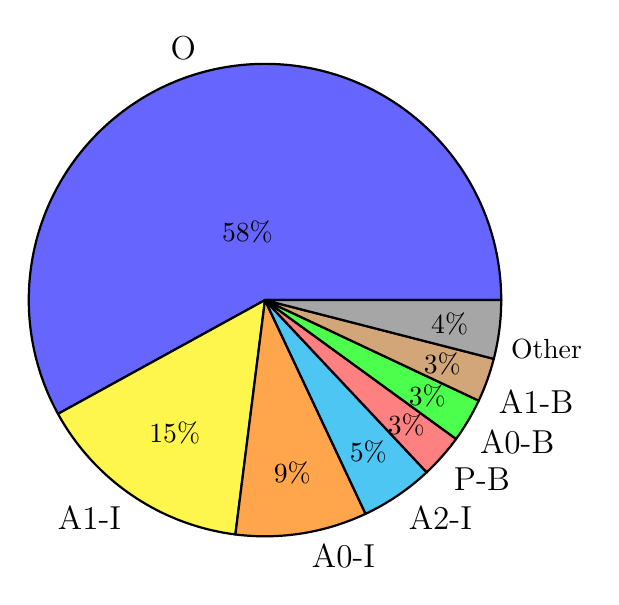
\begin{tikzpicture}
  \pie[color ={blue!60 , yellow!70 , orange!70 , cyan!70, red!50, green!70, brown!70, gray!70}]{58/\oielabel{O}, 15/\oielabel{A1-I}, 9/\oielabel{A0-I}, 5/\oielabel{A2-I}, 3/\oielabel{P-B}, 3/\oielabel{A0-B}, 3/\oielabel{A1-B}, 4/Other}
\end{tikzpicture}
}
\end{scalebox}
\caption{Original label distribution in the Open IE corpus.}
\label{fig:orig_label_dist}
\end{figure}


\begin{figure}[t!]
\centering
%\resizebox{1\columnwidth}{!}{
\begin{scalebox}{0.9}{
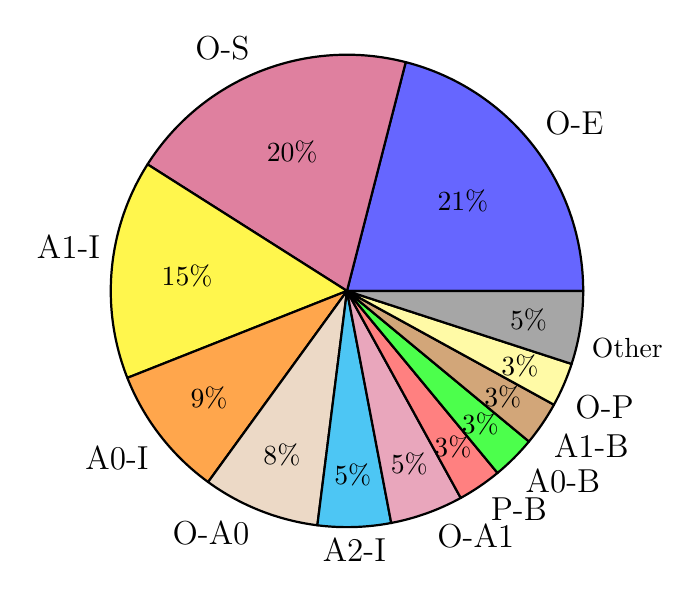
\begin{tikzpicture}
  \pie[color ={blue!60, purple!50, yellow!70 , orange!70 ,  brown!30, cyan!70, purple!35, red!50, green!70, brown!70,
      yellow!35, gray!70}]{21/\oielabel{O-E}, 20/\oielabel{O-S}, 15/\oielabel{A1-I}, 9/\oielabel{A0-I}, 8/\oielabel{O-A0}, 5/\oielabel{A2-I}, 5/\oielabel{O-A1}, 3/\oielabel{P-B}, 3/\oielabel{A0-B}, 3/\oielabel{A1-B}, 3/\oielabel{O-P}, 5/Other}
\end{tikzpicture}
}
\end{scalebox}
\caption{Label distribution after relabeling.}
\label{fig:new_label_dist}
\end{figure}


\subsection{Data Encoding}
\label{sec:encoding}
%% \begin{itemize}
%%   \item We choose to model Open IE as a word level annotation task.

%%   \item We devise a variant on the well known BIO (Beginning, Inside, Outside)  annotation \cite{ramshaw1995text,sang1999representing},
%%   often used in sequence labeling tasks, such as noun phrase chunking, named entity recognition,
%%   or SRL.
%%   This fits our task, as all predicates consist of consecutive, non overlapping span of words.

%%   \item Specifically, each predicate (all verbs, in our case) in the sentence produces an encoding of all of the words
%%   in the sentence relative to their role for the specific target predicate.

%%   \item With regards to a specific target predicate, each word can either be at the start or inside a predicate / argument span, or outside of both.
%%   See Table \ref{tab:oie_examples} for various encoding examples.

%%   \item Each argument is encoded using its index \emph{in the Open IE tuple}.
%%   Note that this encodes semantic information, as these are often rearranged to form
%%   a correct and coherent proposition.
%%   See the last example in Table \ref{tab:oie_examples} in which the order of arguments
%%   in the Open IE tuple deviates from the ordering in the original sentence due to
%%   a relative clause construction (headed by the word ``Brexit'').

%%   \item A special case occurs when a single predicate yields multiple propositions.
%%   This happens in several linguistic and syntactic constructions, such as apposition, co-ordination, or coreference.

%%   \item We handle this by when encoding the predicate by repeating the argument label per the
%%   each tuple it appears in.

%%   \item For example, see the second example in the table shows this phenomenon happening in appositive
%%   construction.

%% \end{itemize}

We choose to model Open IE as a word level annotation task. We follow,  and slightly modify, the well known BIO (Beginning, Inside, Outside)  annotation \cite{ramshaw1995text,sang1999representing},
often used in sequence labeling tasks such as noun phrase chunking, named entity recognition and SRL.
%\todo{notice I changed the terminology to refer consistently to  "predicate", rather that "verb", to make it general}
In our scenario, we annotate a sentence in multiple passes, each time with respect to another targeted predicate within it. Each such target predicate induces an encoding of all other words
in the sentence, which specifies the role of each word with respect to the target predicate.
Concretely, each word can be either at the beginning or inside of either the predicate or an argument span, or outside of both.
%\todo{I'm not sure for the meaning of the following sentence. Why is it important that the predicates are consecutive and non-overlapping? Worth clarifying}
This fits our data, as all our predicates and arguments consist of consecutive, non overlapping spans of words, which BIO labeling is capable of represnting.
See Table \ref{tab:oie_examples} for various encoding examples.

As seen in the table, the encoding identifies each argument by specifying its index (position) in the Open IE tuple.
Note that this ordering captures certain semantic information, as the arguments in a tuple are often rearranged relative to their original order in the sentence in order to form
a correct and coherent proposition when reading the standalone tuple. Thus, an agent would typically be the first argument, a theme the second one and so on, even though the Open IE ordering is looser and less consistent than the pre-defined role labels in SRL.
For instance, see the last example in Table \ref{tab:oie_examples}, in which the order of the arguments
in the Open IE tuple deviates from the ordering in the original sentence due to
a relative clause construction (headed by the word ``Brexit'').

%\todo{Please check that I phrased it properly}
A special case for argument encoding occurs when a single target predicate yields multiple propositions.
This might happen in several linguistic and syntactic constructions, such as apposition, co-ordination and coreference, as illustrated in the second example in the table. As can be seen in the encoding of this example, we assign the same argument index to all arguments in that position, coming from the different propositions headed by the current target predicate. This process is reversed later during decoding, at inference time (Subsection \ref{subsec-inference}).

\subsubsection{Dealing with label imbalance}
%\todo{I wonder if this should be 3.1.1, also fitting the section outline preceding 3.1}
%% \begin{itemize}
%% \item Applying this label scheme on the train partition of the  Open IE data set required the use
%% of 15 labels.
%% Two labels for predicates - \oielabel{P-B}, and \oielabel{P-I}.
%% 12 labels for arguments, as the maximum observed number of arguments was 6, and each of which requires 2 labels.
%% Finally, one label (\oielabel{O}) is used for representing the Outside label.

%% \item Examining the label distribution in the Open IE corpus (Figure \ref{fig:orig_label_dist})
%% reveals a heavy bias towards the \oielabel{O} label.

%% \item This is expected, as most words will not be participate in a predicate or any of the arguments for a given frame.

%% \item Initial experiments showed that this heavy bias towards the Outside label poses a problem.
%% The training process kept converging on a model which predicted the majority class for all words, regardless of their context.

%% \item To cope with this problem, we introduced an artificial division of the of the \oielabel{O}
%% label into @ classes, based on the last observed non-Outside label (i.e., predicate or argument label).
%% In addition, we introduce two more ``Outside'' labels for when the Outside label appeared at the beginning of the sentence (before any non-Outside label was observed)
%% or a the end of it (when these the remainder of the labels are outside of any predicate or argument).
%% For example, revisiting the first example in Table \ref{tab:oie_examples}, our revised annotation would assign the following labels: @

%% \item Recalculating the label distribution with the artificially extended set shows
%% a much more balanced partition (Figure \ref{fig:new_label_dist}.
%% As we will show in Section \ref{sec:evaluation}, this extension indeed enables our model to
%% learn from the variability in the data and converge on more useful weight configurations.

%% \end{itemize}

Applying the above labeling scheme on the train partition of the Open IE data set required the use
of 15 labels:
Two labels for predicates - \oielabel{P-B} and \oielabel{P-I}, and 12 labels for arguments, as the maximum observed number of arguments was 6 and each of which requires 2 labels (Beginning and Inside). Finally, one label (\oielabel{O}) is required for representing the Outside label.

Examining the resulting label distribution in the Open IE corpus (Figure \ref{fig:orig_label_dist})
reveals a heavy bias towards the \oielabel{O} label, corresponding to over half of the words.
This is an expected property of our per-predicate encoding, since each sentence is typically composed of several propositions, headed by different predicates. Accordingly, most sentence words will not be related to any single target predicate. 

Initial experiments showed that this heavy bias towards the Outside label poses a problem for our classification algorithm.
The training process kept converging on a model that predicted the majority class for all words, regardless of their context.
To cope with this problem, we introduced an artificial division of the \oielabel{O}
label into 16 classes. 14 of those correspond to the last observed non-Outside label (i.e., predicate or argument label).
In addition, we introduce two more ``Outside'' labels: \oielabel{O-S} for when the Outside label appeared at the beginning of the sentence (before any non-Outside label was observed)
and \oielabel{O-E} at the end of the sentence (when the remainder of the words are outside of any predicate or argument).
For example, our revisited annotation for the second example in Table \ref{tab:oie_examples} (first proposition) would be:

%% \begin{figure}
%% \ann{The}{A0-B} \ann{president}{A0-I} \ann{claimed}{P-B} \ann{that}{P-I} \ann{he}{P-I} \ann{won}{P-I}
%% \ann{the}{A1-B} \ann{majority}{A1-I} \ann{vote}{A1-I}
%% \end{figure}

\begin{figure}[H]
%  \vspace{-1\baselineskip}x
  \framebox{\parbox{\dimexpr\linewidth-2\fboxsep-2\fboxrule}{
                 \ann{Barack}{A0-B} \ann{Obama}{A0-I} \ann{,}{O-A0} \ann{a}{O-A0} \ann{former}{O-A0} \ann{U.S.}{O-A0} \ann{president}{O-A0} \ann{,}{O-A0} \ann{was}{P-B} \ann{born}{P-I} \ann{in}{P-I} \ann{Hawaii}{A1-B}
}}
%\vspace{-1\baselineskip}
\end{figure}


Following this label manipulation, we recalculate the label distribution and find
a much more balanced partition (Figure \ref{fig:new_label_dist}).
As we will show in Section \ref{sec:evaluation}, this manipulation indeed enables our learning process to
converge on a more useful model.
Previous models have dealt with label bias in various other techniques, which might be better suited
for tasks with smaller label sets. These include, for example:
relabling with BILOU labels \cite{ratinov2009design},
label resampling \cite{estabrooks2004multiple},
or CRF for conditioning current prediction on previous model decisions \cite{baidusrl}.

\subsection{Model Architecture and Feature Extraction}
Given this task formulation and the fact that the sentences are of arbitrary length,
it is appealing to model the task using Recurrent Neural Networks (RNNs).
This approach was proven to be effective in many recent NLP models 
(see \cite{goldberg2015primer} for a recent extensive survey of RNNs in NLP).

%\todo{is it really a deep transducer? In the figure there's only one layer of LSTM in each direction}
Specifically, we use a bi-directional deep LSTM transducer \cite{graves2012sequence},
which takes into account arbitrary length contexts from both past and future words.
The input to the LSTM is a raw sentence and a target predicate (a verb in our implementation),
and its output is a probability distribution, per word, over the possible labels with respect to the target predicate.

The complete architecture of our LSTM model is presented in Figure \ref{fig:architecture}. The input features per word in the sentence are:
\begin{enumerate}
\item
300 dimensional word embedding vectors for both the current word and the target predicate, taken from the same embedding space.
That is, a predicate word would have the same
representation whether it is considered as the target predicate or not.
%\todo{the commented text doesn't seem needed, it's quite clear}
% This happens in case where there is more than one predicate in the sentence as in example @ in
% Table \ref{tab:oie_examples}.

\item 5 dimensional embedding of the part of speech of the current word and the target predicate, and
\item The position index of the word and the target predicate in the sentence.

\end{enumerate}
%% \todo{In the figure each word, and the predicate, split to two circles and it's not clear what each of them stands for. I thought they represent the embedding components, but there are three components.}
%\todo{Is it OK not to give the network equations?}

\subsection{Inference}
\label{subsec-inference}

%% \begin{itemize}
%% \item During inference, we decode Open IE extractions from the most probable label assignment for each word,
%% as predicted by our LSTM.
%% \item We do by recovering coherent spans of arguments (ones which start with \label{B-A_i}), and producing an extraction per each combination in the Cartesian product of arguments.
%% \item Multiple proposition per target predicate therefore occur when there is more than one instantiation of an argument type.
%% \item For example: @
%% \end{itemize}

%\todo{check and complete details if neded, such as POS tool you used}
During inference, we first identify all verbs in the sentence using a POS tagger and generate an input instance for the LSTM transducer per each verb.
For a given instance, we regard the most probable LSTM label assignment for each word as the predicted encoding for the sentence, and decode Open IE extractions from these labels.
We do so by recovering coherent spans for the predicate and arguments, starting with a Beginning label (e.g., \oielabel{A1-B}) and continuing with corresponding Inside labels.
Then, if each argument index occurs only once we simply generate a single extraction tuple headed by the predicate and including all arguments. If some argument indexes appear more than once, this corresponds to the case where a single predicate generates multiple extractions, as discussed at the encoding phase (end of Subsection \ref{sec:encoding}). Accordingly, we generate multiple extraction tuples, each one headed by the target predicate and containing one possible combination of arguments, choosing one argument for each position index. Overall, decoding reverses the encoding process, this time from BIO labels to extractions, as illustrated in Table \ref{tab:oie_examples}.


\paragraph{Assigning extraction confidence}
As discussed in Section \ref{sec:background}, it is beneficial for Open IE systems to associate a confidence value with each predicted extraction.
In our case, the LSTM assigns a probability to each label prediction, for each word.
We experimented with several heuristics to combine these predictions to an extraction level confidence metric.
The best performance on the development set was achieved by multiplying the word-level probabilities of each
of the elements participating in the extraction.\footnote{Other variants we tried were taking the maximum or
minimum observed probability, but that performed worse.}

We note that this metric clearly prefers shorter extractions.
While this is beneficial for the task of Open IE, which aims to reduce proposition span, an interesting
avenue for future research is developing a more principled way of assigning confidence scores to extractions.


\subsection{Implementation details}
We implemented the bi-LSTM transducer model using the \keras\ framework \cite{chollet2015} with a \tensorflow\ backend \cite{tensorflow2015-whitepaper}.
We use 3 layers of stacked bi-LSTMs, where each LSTM cell is composed of 128 hidden units
with a linear rectifier (ReLU) \cite{nair2010rectified} activation function.
Training was done on 100 epochs, in mini batches of 50 samples, with 10\% word level
dropout.
Word embeddings were initialized using the pre-trained embeddings computed in \newcite{pennington2014glove}, with loss propagating back to the word representation during training, hopefully
allowing them to assimilate a task-specific representation.

Finally, we use the average perceptron part-of-speech tagger (as implemented in spaCy\footnote{\url{https://spacy.io}})
to predict the part of speech for both feature computation and predicate identification (identifying verbs).


\section{Evaluation}
\label{sec:evaluation}
%% \begin{itemize}
%% \item We implemented the bi-LSTM transducer model using the \keras\ framework \cite{chollet2015} with a \tensorflow\ backend \cite{tensorflow2015-whitepaper}.
%%   We use 3 layers of stacked bi-LSTMs, where LSTM cell is composed of @ hidden units.
%%   for the LSTM we use

%%   \item Dimensions of layers
%%   \item activation functions
%%   \item Average perceptron part of speech tagging (as implemented in spaCy\footnote{\url{https://spacy.io}}
%%   \item Word embedding intialization using the pre-trained embeddings computed in
%%     \newcite{pennington2014glove}.
%% \end{itemize}

When evaluating Open IE it is desired to allow some room for flexibility when comparing against gold annotated extractions, for several reasons.
First, as we mentioned previously, current prominent Open IE systems were developed without a large reference
corpus. Following, this created some deviation in design and representation choices between the systems.
For example, ClausIE chooses to predict only extractions with two arguments (versus n-ary extractions in the other systems), and PropS includes prepositions as part of the predicate while Open IE4 posits them in the respective
argument slot.

Second, like other tasks that require subtle semantic decisions, such as summarization or machine translation,
there are often several possible  extractions that might be regarded as correct, and we do not want to penalize systems for not
recovering the specific choice made in the gold corpus.
For example, for the sentence \sent{The sheriff standing against the wall spoke in a very soft voice} the two following
extractions can be considered acceptable: \extraction{The Sheriff}{spoke}{in a soft voice},
\extraction{The sheriff standing against the wall}{spoke}{in a very soft voice}

To account for  this variance in predictions, we follow \newcite{hequestion} and \newcite{Stanovsky2016EMNLP} which judge an argument as correct if and only if it includes the \emph{syntactic head} of the gold argument.\footnote{We make use of the test suite published in \url{https://github.com/gabrielStanovsky/oie-benchmark}}
This would accept both variations of the previous example.
Note that this relaxed matching allows for fair comparison with rule-based systems which did not use a training
set to fit their prediction according to a strict matching function.

\subsection{Results}

\pgfplotsset{
	compat=1.5, 
	label style={font=\footnotesize},
	legend style={font=\footnotesize},
	every tick label/.append style={font=\tiny},
}



\begin{figure}  

\vspace{-2mm}
\centering

\begin{tikzpicture}
  \begin{axis}[
  ybar,
  bar width=2pt,
  xtick=data,% crucial line for the xticklabels directive
   xticklabels from table={../evaluations/figures/joint/predicate/auc.dat}{system}
  ]
        \addplot[red,mark size=0pt] table [x=auc] {../evaluations/figures/joint/predicate/auc.dat};
  \end{axis}
\end{tikzpicture}

\caption{AUC Predicate identification @}
\label{fig:rascal}



\end{figure}

\pgfplotsset{
	label style={font=\footnotesize},
	legend style={font=\footnotesize},
	every tick label/.append style={font=\tiny},
        every node near coord/.style={font=\tiny},
        every axis plot/.append style={line width = 0.6pt}
}



\begin{figure}[!ht]
    \centering
\begin{tikzpicture}
%%% ALL
\begin{axis}[
	xlabel=Recall,
        xticklabel pos=right,
	ylabel=Precision,
%	ymin=0,
	ymax=1,
        xmin=0,
        xmax=1,
	%ytick distance=.1,
%	height=0.25\textheight,
	width=0.33\textwidth,
	axis lines=left,
	%% legend entries={RnnOIE,OpenIE-4,PropS,ClausIE},
	%% legend style={draw=none,font=\tiny,at={(1,0.01)}, anchor=south east},
         /pgf/number format/.cd,
        1000 sep={}
]
\addplot[color1,mark size=0pt] table [x=Recall,y=Precision] {../../evaluations/figures/joint/RnnOIE.dat} node[right,pos=1] {\tiny RnnOIE};
\addplot[color2,mark size=0pt] table [x=Recall,y=Precision] {../../evaluations/figures/joint/OpenIE-4.dat} node[left,pos=1] {\tiny OpenIE-4};
\addplot[color3,mark size=0pt] table [x=Recall,y=Precision] {../../evaluations/figures/joint/PropS.dat} node[below,pos=0.7] {\tiny PropS};
\addplot[color4,mark size=0pt] table [x=Recall,y=Precision] {../../evaluations/figures/joint/ClausIE.dat} node[above,pos=1] {\tiny ClausIE};
\end{axis}
\end{tikzpicture}
%% \renewcommand{\thesubfigure}{a}
%% \subfloat[\small{Full Open-IE: PR and AUC.}]{
%% \label{fig:prop}
    \begin{tikzpicture}
  \begin{axis}[
  width = 0.4\textwidth,
  height=5cm,
  xbar,
  xmax = 0.49,
  bar width=2pt,
  xtick= \empty,
  ytick=data,% crucial line for the xticklabels directive
   yticklabels from table={../../evaluations/figures/joint/auc.dat}{system},
nodes near coords,
nodes near coords align={horizontal}
  ]
        \addplot[draw=blue,fill=blue!80!white,mark size=0pt] table [x=auc, y expr=\coordindex] {../../evaluations/figures/joint/auc.dat};
  \end{axis}
\end{tikzpicture}
%% $\;$
%% \renewcommand{\thesubfigure}{b}
%% \subfloat[\small{Predicate extraction: PR and AUC.}]{
%% \label{fig:pred}
%%     \begin{tikzpicture}
%%   \begin{axis}[
%%   width = 0.3\textwidth,
%%   height=3cm,
%%   xbar,
%%   xmax = 0.62,
%%   bar width=2pt,
%%   ytick=data,% crucial line for the xticklabels directive
%%    yticklabels from table={../evaluations/figures/joint/predicate/auc.dat}{system},
%% nodes near coords,
%% nodes near coords align={horizontal}
%%   ]
%%         \addplot[draw=blue,fill=blue!80!white,mark size=0pt] table [x=auc, y expr=\coordindex] {../evaluations/figures/joint/predicate/auc.dat};
%%   \end{axis}
%% \end{tikzpicture}

%%     }
%%     $\;$
%% \renewcommand{\thesubfigure}{c}
%% \subfloat[\small{Argument extraction: PR and AUC.}]{
%% \label{fig:arg}
%%     \begin{tikzpicture}
%%   \begin{axis}[
%%   width = 0.3\textwidth,
%%   height=3cm,
%%   xbar,
%%   xmax = 0.71,
%%   bar width=2pt,
%%   ytick=data,% crucial line for the xticklabels directive
%%    yticklabels from table={../evaluations/figures/joint/arguments/auc.dat}{system},
%% nodes near coords,
%% nodes near coords align={horizontal}
%%   ]
%%         \addplot[draw=blue,fill=blue!80!white,mark size=0pt] table [x=auc, y expr=\coordindex] {../evaluations/figures/joint/arguments/auc.dat};
%%   \end{axis}
%% \end{tikzpicture}
%% }
%%     %% \qquad
%%     %% \subfloat[Figura 3]{
%%     %%     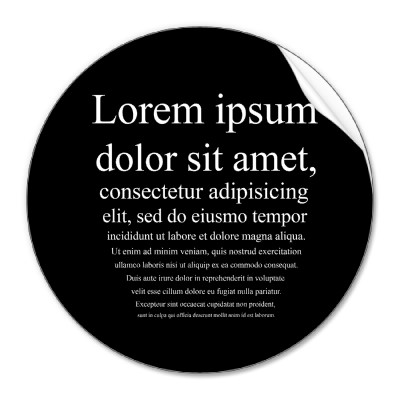
\includegraphics[width=0.4\columnwidth]{./figures/lorem-ipsum.jpg}
%%     %% }
%%     \caption{Precision-recall curves of the different systems on Open IE's subtasks (top),
%%     and corresponding areas under the curve (bottom)  -- complete Open IE (predicate-argument extraction) (\ref{fig:prop}),
%%     predicate extraction (\ref{fig:pred}), and argument extraction (\ref{fig:arg}).
%%     See details in Section \ref{sec:analysis}.
%%     }
%%     \label{fig:subfigname}
\end{figure}



\pgfplotsset{
	compat=1.5, 
	label style={font=\footnotesize},
	legend style={font=\footnotesize},
	every tick label/.append style={font=\tiny},
}



\begin{figure}  

\vspace{-2mm}
\centering
\begin{tikzpicture}
\begin{axis}[
	xlabel=Recall,
	ylabel=Precision,
	ymin=0,
	ymax=1,
        xmin=0,
        xmax=1,
	%ytick distance=.1,
	height=0.25\textheight,
%	width=\columnwidth,
	axis lines=left,
	legend entries={RnnOIE,OpenIE-4,PropS,ClausIE},
	legend style={draw=none,font=\tiny,at={(1,0.01)}, anchor=south east},
         /pgf/number format/.cd,
        1000 sep={}
]

\addplot[red,mark size=0pt] table [x=Recall,y=Precision] {../evaluations/figures/joint/predicate/RnnOIE.dat};
\addplot[brown,mark size=0pt] table [x=Recall,y=Precision] {../evaluations/figures/joint/predicate/OpenIE-4.dat};
\addplot[orange,mark size=0pt] table [x=Recall,y=Precision] {../evaluations/figures/joint/predicate/PropS.dat};
\addplot[blue,mark size=0pt] table [x=Recall,y=Precision] {../evaluations/figures/joint/predicate/ClausIE.dat};

\end{axis}
\end{tikzpicture}
\caption{Predicate identification @}
\label{fig:rascal}



\end{figure}

\pgfplotsset{
	compat=1.5, 
	label style={font=\footnotesize},
	legend style={font=\footnotesize},
	every tick label/.append style={font=\tiny},
}



\begin{figure}  

\vspace{-2mm}
\centering
\begin{tikzpicture}
\begin{axis}[
	xlabel=Recall,
	ylabel=Precision,
	ymin=0,
	ymax=1,
        xmin=0,
        xmax=1,
	%ytick distance=.1,
	height=0.25\textheight,
%	width=\columnwidth,
	axis lines=left,
	legend entries={RnnOIE,OpenIE-4,PropS,ClausIE},
	legend style={draw=none,font=\tiny,at={(1,0.01)}, anchor=south east},
         /pgf/number format/.cd,
        1000 sep={}
]

\addplot[red,mark size=0pt] table [x=Recall,y=Precision] {../evaluations/figures/joint/arguments/RnnOIE.dat};
\addplot[brown,mark size=0pt] table [x=Recall,y=Precision] {../evaluations/figures/joint/arguments/OpenIE-4.dat};
\addplot[orange,mark size=0pt] table [x=Recall,y=Precision] {../evaluations/figures/joint/arguments/PropS.dat};
\addplot[blue,mark size=0pt] table [x=Recall,y=Precision] {../evaluations/figures/joint/arguments/ClausIE.dat};

\end{axis}
\end{tikzpicture}
\caption{Arguments @}
\label{fig:rascal}



\end{figure}

\pgfplotsset{
	compat=1.5, 
	label style={font=\footnotesize},
	legend style={font=\footnotesize},
	every tick label/.append style={font=\tiny},
}



\begin{figure}  

\vspace{-2mm}
\centering
\begin{tikzpicture}
\begin{axis}[
	xlabel=Recall,
	ylabel=Precision,
	ymin=0,
	ymax=1,
        xmin=0,
        xmax=1,
	%ytick distance=.1,
	height=0.25\textheight,
%	width=\columnwidth,
	axis lines=left,
	legend entries={Seen in train,Unseen in train},
	legend style={draw=none,font=\tiny,at={(1,0.01)}, anchor=south east},
         /pgf/number format/.cd,
        1000 sep={}
]

\addplot[cyan, mark size=0pt] table [x=Recall,y=Precision] {../evaluations/only_in_test/seen.dat};
\addplot[purple,mark size=0pt] table [x=Recall,y=Precision] {../evaluations/only_in_test/unseen.dat};

\end{axis}
\end{tikzpicture}
\caption{Seen vs. Unseen @}
\label{fig:rascal}



\end{figure}



% accuracy and attention comparison figures

\begin{figure*}[t!]

  \centering
  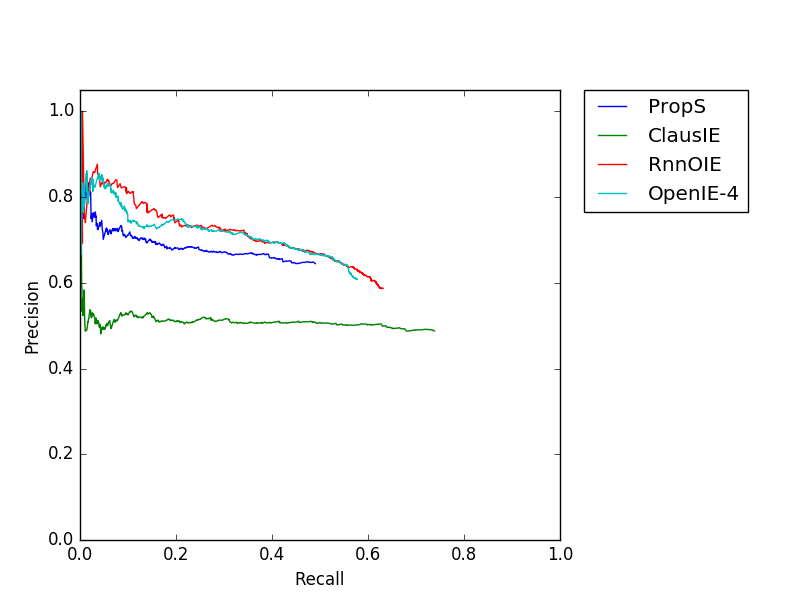
\includegraphics[width=.5\textwidth]{figures/joint/pr}\hfill
  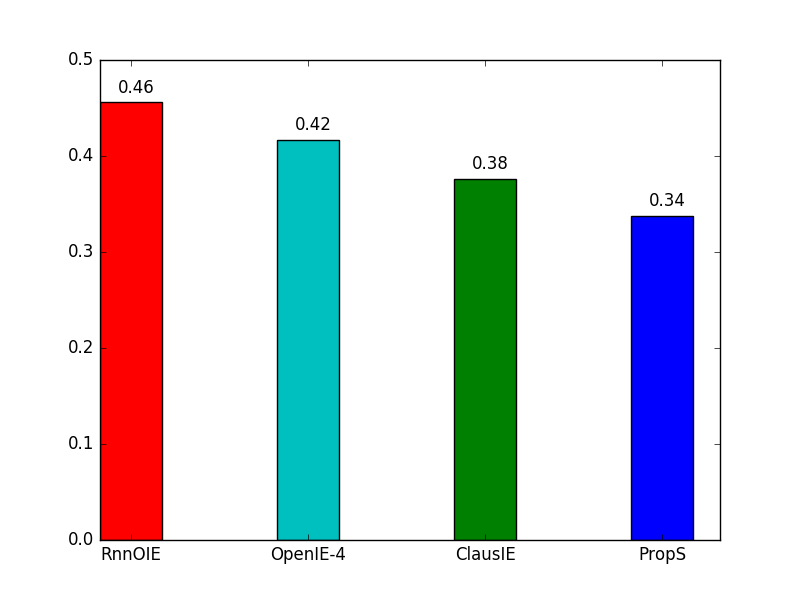
\includegraphics[width=.5\textwidth]{figures/joint/auc}

  \caption{Precision-Recall curve (left) and respective area under the curve (right) for the different systems.}
  \label{fig:evaluation}

\end{figure*}


%% \begin{figure*}[t!]

%%   \centering
%%   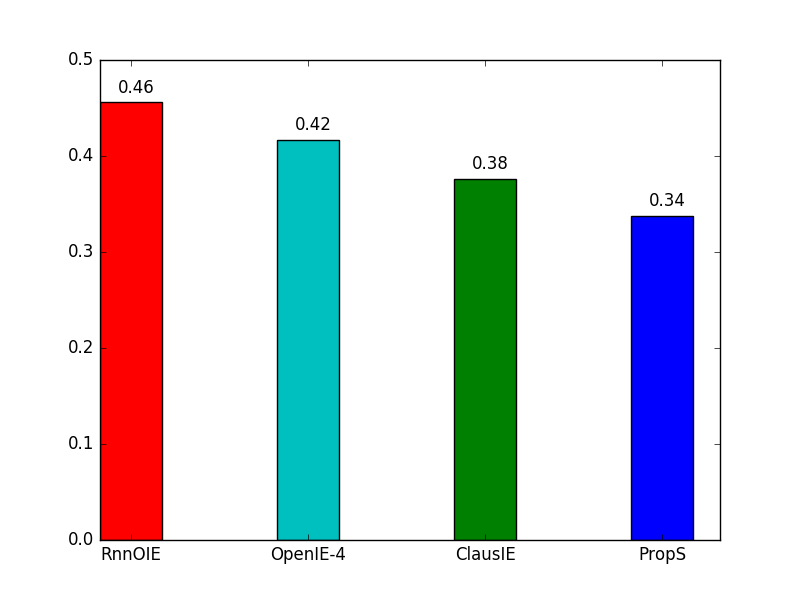
\includegraphics[width=.3\textwidth]{figures/joint/auc}\hfill
%%   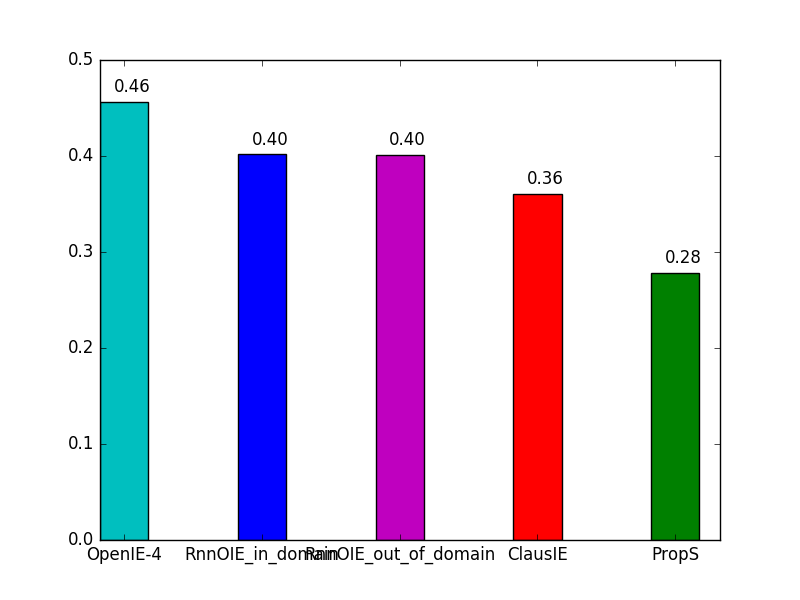
\includegraphics[width=.3\textwidth]{figures/newswire/auc}\hfill
%%     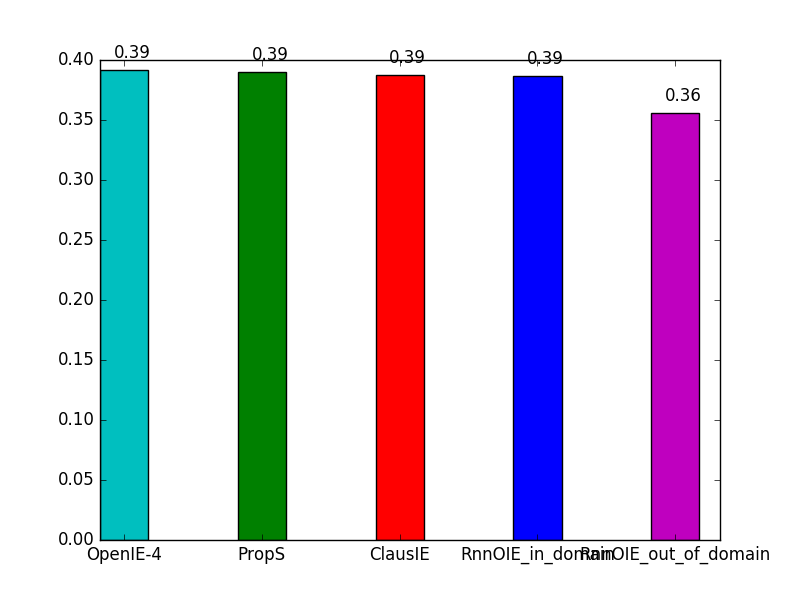
\includegraphics[width=.3\textwidth]{figures/wiki/auc}

%%   \caption{Area under the PR - curves for the entire test corpus (left), Newswire (middle), and Wikipedia (right).}
%%   \label{fig:figure3}

%% \end{figure*}



%% \begin{figure*}[!hb]

%%   \centering

%%   \begin{minipage}[b]{.12\textwidth}
%%     \begin{center}
%%       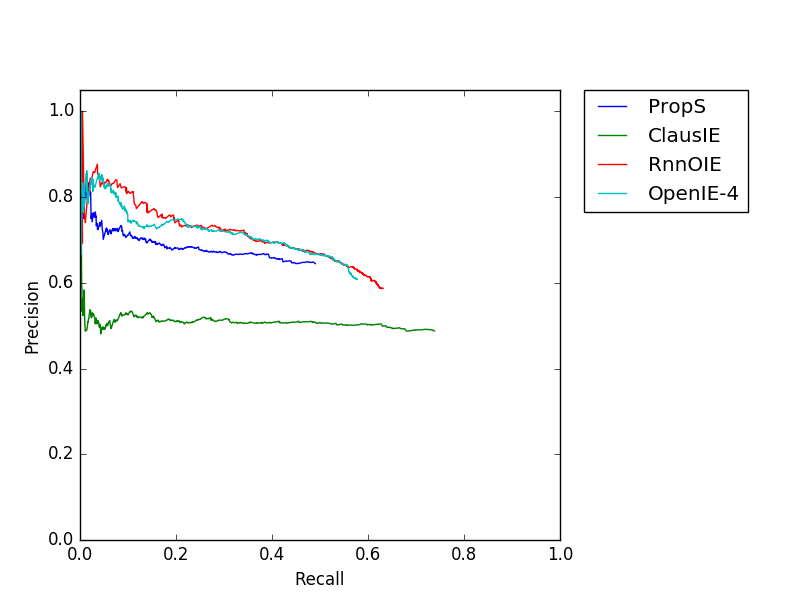
\includegraphics[width=\textwidth]{figures/joint/pr}
%%       \caption {Precision-recall curve on the full test partition}
%%       \label{fig:alignments}
%%     \end{center}
%%   \end{minipage}

%%   \begin{minipage}[b]{0.12\textwidth}
%%     \begin{center}
%%       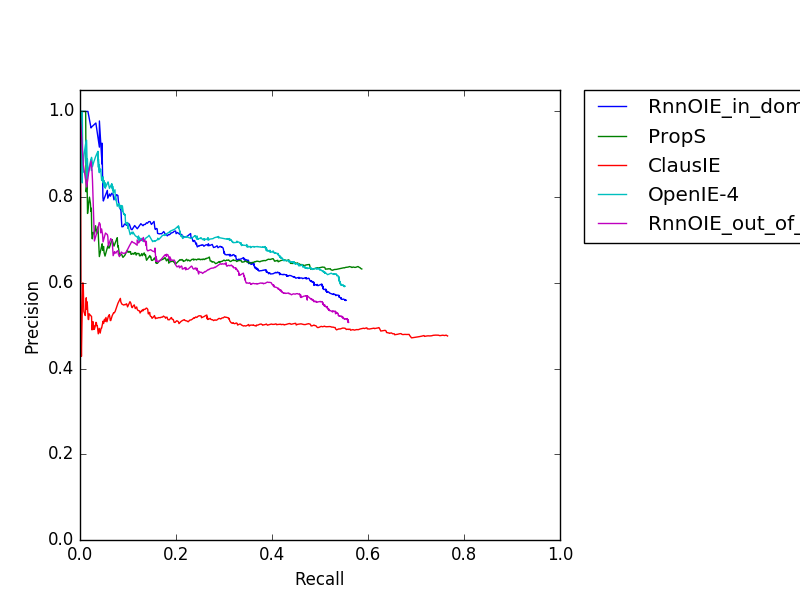
\includegraphics[width=\textwidth]{figures/wiki/pr}
%%       \caption {Precision-recall curve on the Wikipedia test partition}
%%       \label{fig:alignments}
%%     \end{center}
%%   \end{minipage}

%%   \begin{minipage}[b]{0.12\textwidth}
%%     \begin{center}
%%       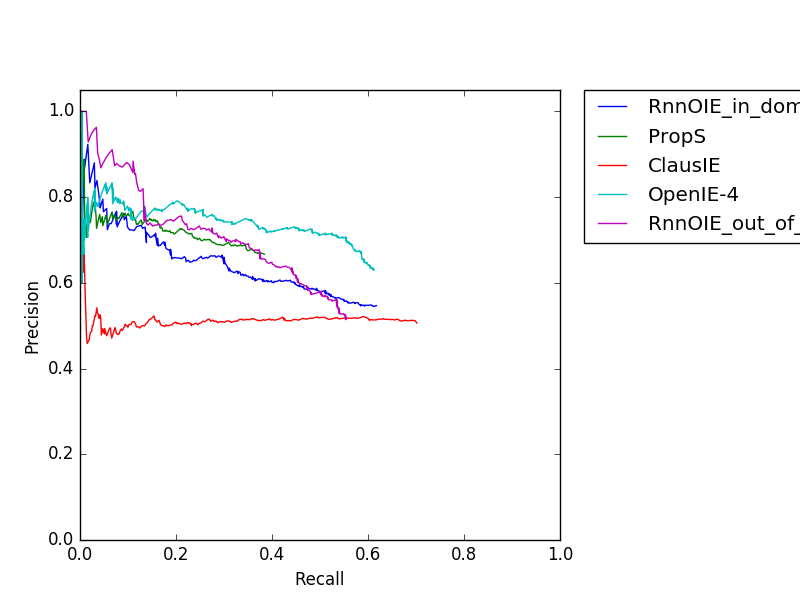
\includegraphics[width=\textwidth]{figures/newswire/pr}
%%       \caption {Precision-recall curve on the newswire test partition}
%%       \label{fig:alignments}
%%     \end{center}
%%   \end{minipage}


%% \end{figure*}


The Precision-Recall (PR) curve of our model (marked RnnOIE) is shown in Figure \ref{fig:evaluation},
using the soft matching function discussed above.
For comparison, we plot the performance of the top performing systems evaluated in \cite{Stanovsky2016EMNLP} on the same corpus. We note that these are very strong baseline systems, which are the result of over a decade of research.

RnnOIE outperforms the other systems in terms of precision on most of the recall range, and comes in second after (the much less precise) ClausIE in terms of maximum obtained recall (.63 versus .74).
Superior precision performance is especially attractive for
applications that employ Open IE over large amounts of data, in which a high degree of data redundancy is expected, such as in different news reports of the same event.

Following, the Area Under the PR-Curve (AUC) shows that overall our system
produces the best combination of aggregated precision and recall with a statistically significant margin over
the other systems. In scalar terms of the AUC, our improvement over state-of-the-art is similar in magnitude to previous
advancements in the field (4 points).


%\todo{it's worth mentioning the statistical test used}

%% \begin{itemize}
%% \item Figures:
%%   \begin{itemize}
%%   \item Optimizing precision vs. recall.
%%   \item In \& Out of domain?
%%   \item Number of extractions per system
%%   \item Check whether its common to report ``intrinsic'' numbers
%%   \end{itemize}
%% \end{itemize}

\begin{table}[tb!]
  \centering
  \resizebox{1\columnwidth}{!}{
    \begin{tabular}{@{}lrrr@{}}
      \toprule
      \multirow{2}{*}{\textbf{System}} & \multicolumn{1}{l}{\multirow{2}{*}{\textbf{\# Extractions}}} & \multicolumn{1}{l}{\multirow{2}{*}{\textbf{Arg. per Prop.}}} & \multicolumn{1}{l}{\multirow{2}{*}{\textbf{Words per Arg}}} \\
      & \multicolumn{1}{l}{} & \multicolumn{1}{l}{} & \multicolumn{1}{l}{} \\ \midrule
      Gold & 1730 & 2.45 & 26.91 \\ \midrule
      ClausIE & 2768 & 2.00 & 28.89 \\
      Open IE4 & 1793 & 3.07 & 22.75 \\
      PropS & 1551 & 2.68 & 29.00 \\
      RnnOIE & 1993 & 3.19 & 23.40 \\ \bottomrule
      \end{tabular}
  }
  \caption{Output statistics of the different systems.}
  \label{tab:output_stats}
  \end{table}


\subsection{Analysis}
We describe several observations about the performance of the evaluated systems.

\paragraph{RnnOIE and Open IE4 produce shorter arguments.}
In Table \ref{tab:output_stats} we examine some properties of the output of different systems compared to the corresponding gold data.
This allows us to gain some insight into the performance of the systems.
For example, we can see that the best performing systems (RnnOIE and OpenIE4), tend to produce
more arguments, each of which tending to be shorter in terms of word count.
This observation fits the \emph{minimality} principle of Open IE, discussed in Section \ref{sec:background}.
Comparing to the same properties in the gold data set (first row), we can see that both systems
tend to overproduce and over-shorten their arguments.
% Compared to 2.45 arguments of 26.91 word length in average for the gold data set,
% RnnOIE and Open IE4 produce 3.07 and 3.19 arguments of word length 23.4 and 22.75 in average, respectively.

\paragraph{RnnOIE is able to generalize to unseen predicates.}
We analyze the extent to which our model overfits for the predicates seen during training, that is, whether it achieves good performance by memorizing specific patterns for these predicates.
To that end we have split the propositions in the gold and predicted test set into two corresponding partitions, namely ``seen'' and ``unseen'',
based on whether the predicate lemma appears in the training set or not.
The ``unseen'' part of the test set contains 145 unique predicate lemmas, constituting
24\% out of a total of 590 unique predicate lemmas in the entire test set.
Furthermore, it is composed of a total of 148 propositions (7\% out of 1993 in the entire test).
%% \todo{the above sentence isn't so clear, not sure what you meant to say. Do you refer to the fact that in 148 unseen propositions there were 145 different predicates? This isn't that surprising - events not seen in training are rare and are likely to be singletons in test. If that's the case maybe you can drop this sentence on the variability, not sure if it contributes to the main point here on unseen}

Following, we tested each of the predicted test partitions against its corresponding gold
counterpart.
The resulting PR curves (Figure \ref{fig:unseen}) depict overall good performance on the ``unseen'' partition,
We note, however, that the ``seen'' part is much larger, constituting roughly 93\% of the test data.
Overall, this indicates that the model indeed generalizes beyond the memorization of specific predicate templates, as
it managed to predict extractions for unseen predicates with good accuracy.

\begin{figure}[tb!]

  \centering
    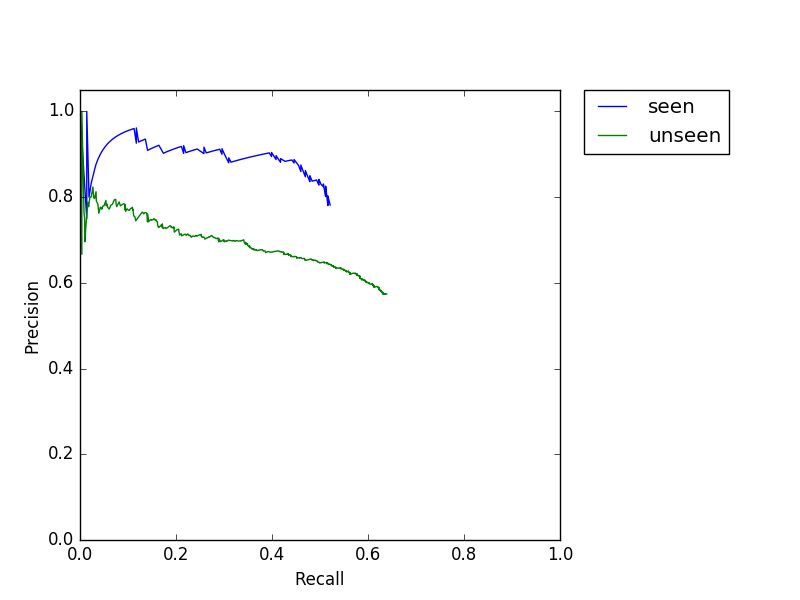
\includegraphics[width=1\columnwidth]{figures/uniq_test_pr}

  \caption{Performance of our model on seen versus unseen test predicates.}
  \label{fig:unseen}

\end{figure}


%% \begin{itemize}
%% \item Performace on ``core'' arguments vs. ``adjuncts''
%% \item Standard error analysis: Sample 50 FN and 50 FP
%% \item Check what number of predicates are unseen in the test in each of these and do they affect performance
%% \end{itemize}


\section{Related Work}
\label{sec:related}
As our model is the first supervised method for Open IE, we compare it here to related work in supervised semantic role labeling (SRL), which, as mentioned throughout the paper,  bears a strong similarity to Open IE.
In particular, we will focus on the recent state-of-the-art deep neural networks models for SRL presented in \cite{baidusrl} and \cite{RothLapata16}.

\newcite{baidusrl} design an end-to-end model for SRL, taking as input the raw text
without any prerequisite NLP annotation (not relying for example on 
syntactic parsing, like some other SRL methods).
Their input is composed of a raw sentence and a target predicate.
In comparison, we take as input only the raw sentence while using a part-of-speech tagger to identify verbal predicates.

Their model encodes the data using the standard BIO annotation,
  and, similarly to our approach, annotates each word's relation to
  a target predicate.
  In particular, each word can either be at the Beginning or Inside of: a frame-specific SRL core argument span
  (\oielabel{B-A\_i}, \oielabel{I-A\_i}), a non-core role (e.g., \oielabel{B-AM-LOC} for locations),
  or a single-word predicate (\oielabel{B-V}).
  In addition, the Outside label (\oielabel{O}) is used to indicate that
  a word does not take part in the current proposition.
  We use a more elaborate encoding scheme (Section \ref{sec:encoding}) to cope with label bias.
  While the label distribution is not discussed in their paper,
  it is probable to assume that this is a lesser problem for SRL annotation,
  since its arguments span across full syntactic constituents and are therefore longer than Open IE arguments, leaving fewer Outside words.

  Further, in terms of modeling, their method also uses a word-level LSTM transducer, but with different features than ours.
  Their word features are: (1) the current word's embedding, (2) the predicate and its context's embedding,
  and (3) a binary feature indicating whether the word is in ``close'' proximity to the predicate word (i.e., less than two words separate them).
  In comparison, our features are the word and predicate embedding (without its context), the
  embedding of their part-of-speech, and the position index of both in the sentence.

  In addition, \newcite{baidusrl} use a Conditional Random Field (CRF) \cite{crf} classifier on top of
  the LSTM as the final prediction stage.
  CRFs can take previous predictions as features for the current predicted label. This is useful for sequence labeling
  tasks, as previously assigned labels will affect the currently predicted label. For example, \oielabel{I-A1} typically follows \oielabel{B-A1}.
  Using a CRF in our model fell out of scope for the current work, as we preferred focusing
  on the novel, task-specific, challenges in devising a supervised model for Open IE. These included encoding and decoding for Open IE, dealing with label bias and computing a confidence score. Testing different extensions of our model, such as an additional CRF layer, is left for future work.

  Finally, \newcite{RothLapata16} take a different and more complex approach for modeling SRL.
  They design a pipeline, composed of 3 components: (1) syntactic dependency parsing,
  (2) predicate identification and disambiguation, and (3) argument identification and classification.
  One of their main novelties is using a new embedding for the dependency path between a predicate
  and its potential arguments, as a feature for argument classification.

  %% In terms of evaluation, it seems hard to compare the performance
  %% of these two systems, as each uses a different test set; \newcite{baidusrl} use the datasets published in the shared tasks of CoNLL-2005 \cite{SRL}
  %% and CoNLL 2012 \cite{pradhan2012conll} while \newcite{RothLapata16} use the dataset published in the CoNLL-2009 shared task \cite{hajivc2009conll}.




%% In particular, we will focus on two recent models which are the current state of the art.
%% the basis of this work is the deep neural network sRL model of \cite{baidusrl}.

%% SRL and Open IE have been defined with different objectives. Particularly, SRL identifies argument role labels, which is not addressed in Open IE.
%% Yet, the two tasks overlap as they both need to recover predicate-argument structures in sentences. We now examine the above Open IE requirements and suggest that while they are
%% only partly embedded within SRL structures, they can be fully recovered from QA-SRL.

%% Asserted (matrix) propositions appear in SRL as non-embedded predicates (e.g., \pred{succeeded} in the \sent{Sam succeeded to convince John}).
%% However, SRL's predicates are grounded to a lexicon such as PropBank \cite{propbank} or FrameNet \cite{framenet}, which violates the \emph{completeness and open lexicon} principle.
%% Further, in contrast to the \emph{minimal propositions} principle, arguments in SRL annotations are inclusive, each marked as full subtrees in a syntactic parse.

%% Yet, QA-SRL seems to bridge this gap between traditional SRL structures and Open IE requirements.
%% Its predicate vocabulary is open,
%% and its question-answer format solicits \emph{minimal propositions}, as was found in a recent study by \cite{2016stanovskyACL}.
%% This correlation suggests that the QA-SRL methodology is in fact also an attractive means for soliciting Open IE extractions from non-experts annotators.
%% %Evidently, it enables us to automatically derive high quality Open IE annotations from existing QA-SRL gold annotations.
%% Evidently, it enables automatically
%% deriving high quality Open IE annotations from (current or future) QA-SRL gold annotations, as described in the following section


\section{Conclusions and Future Work}
\label{sec:conclusions}
We presented the first supervised model for Open IE,
which uses of the recently published large scale corpus for the task \cite{Stanovsky2016EMNLP}.
We model the task as a word-transducing problem, and presented solutions and
adjustments for various task-specific challenges: the encoding-decoding of Open IE instances, while providing a relabeling scheme which alleviates an inherent label-bias, a metric for computing the confidence of an extraction,
and applied a bi-LSTM transducer which follows state-of-the-art models for supervised SRL.
We tested this model against very strong baselines consisting of the current top performing Open IE systems, and
found that it is superior in terms of overall aggregated precision and recall.
In future work, we plan to extend this model to include a more principled learning of the confidence metric,
as well as to extend it beyond non-verbal predicates, which first require supporting supervised
data sets for non-verbal Open IE.
\bibliography{bib}
\bibliographystyle{emnlp_natbib}

\end{document}
